\documentclass[a4paper,twoside]{article}

\usepackage{epsfig}
\usepackage{subcaption}
\usepackage{calc}
\usepackage{amssymb}
\usepackage{amstext}
\usepackage{amsmath}
\usepackage{amsthm}
\usepackage{multicol}
\usepackage{pslatex}
\usepackage{apalike}
\usepackage{algorithm2e}
\usepackage[bottom]{footmisc}
\usepackage{tikz}
\usepackage{booktabs}
\usepackage[utf8]{inputenc}
\usepackage[acronym]{glossaries}
\usepackage{SCITEPRESS}     % Please add other packages that you may need BEFORE the SCITEPRESS.sty package.

\newacronym{crp}{CRP}{clinical research professional}
\newacronym{ehr}{EHR}{electronic health record}
\newacronym{ai}{AI}{artificial intelligence}
\newacronym{ml}{ML}{machine learning}
\newacronym{hcai}{HCAI}{Human-Centered Artificial Intelligence}
\newacronym{hgml}{HGML}{Human-Guided Machine Learning}
\newacronym{automl}{AutoML}{automated machine learning}
\newacronym{hci}{HCI}{human-computer interaction}
\newacronym{gui}{GUI}{graphical user interface}
\newacronym{llm}{LLM}{large language model}
\newacronym{aws}{AWS}{Amazon Web Services}
\newacronym{dl}{DL}{deep learning}
\newacronym{rag}{RAG}{retrieval-augmented generation}
\newacronym{nlp}{NLP}{natural language processing}
\newacronym{aucroc}{AUC-ROC}{area under the curve - receiver operating characteristic}
\newacronym{rmse}{RMSE}{root mean squared error}
\newacronym{mae}{MAE}{mean absolute error}

\newacronym{insuml}{InsuML}{Interactive Support for Non-Expert Users in Machine Learning}

\newacronym{shap}{SHAP}{Shapley additive explanations}
\newacronym{lime}{LIME}{local interpretable model-agnostic explanations}
\newacronym{xai}{XAI}{explainable artificial intelligence}

\makeglossaries

\begin{document}

\title{A Methodology for Evaluating Human-Guided Machine Learning Tools under Human-Centered Artificial Intelligence Criteria: Application to InsuML}

\author{\authorname{Diego García-Prieto\sup{1}\orcidAuthor{0000-0002-7461-2961}, Camilo Palazuelos\sup{1}\orcidAuthor{0000-0003-4132-9550} and Rafael Duque\sup{1}\orcidAuthor{0000-0001-8636-3213}}
\affiliation{\sup{1}Department of Mathematics, Statistics and Computer Science, University of Cantabria, Avenida de Los Castros s/n, Santander, Spain}
\email{\{diego.garciaprieto, camilo.palazuelos, rafael.duque\}@unican.es}
}

\keywords{Human-Centered Artificial Intelligence, Human-Guided Machine Learning, Human-Computer Interaction, AutoML}

% Revisar
\abstract{Human-Guided Machine Learning (HGML) proposes actively integrating expert knowledge into the Machine Learning (ML) lifecycle. However, the evaluation of HGML tools under Human-Centered Artificial Intelligence (HCAI) criteria remains scarce in the literature, and no established methodology exists for conducting such evaluations in a systematic and reproducible manner. This paper makes two contributions: first, it proposes a structured methodology for evaluating HGML tools under HCAI criteria, operationalizing the two-dimensional HCAI framework into concrete pipeline phases, responsibility assignment criteria and a four-step evaluation procedure formalized as an HCAI-HGML Compliance Matrix; second, it applies this methodology to InsuML, an HGML tool designed for users without Artificial Intelligence (AI) expertise. Results demonstrate that InsuML achieves a genuine balance between high automation and high human control, materializing the HCAI framework principles through concrete design decisions: tab-based guided navigation, a pre-training configuration summary functioning as prospective transparency mechanism, and interpretable visualizations. The comparison with existing HGML proposals reveals that InsuML is the only evaluated proposal that combines full pipeline coverage, operational software implementation, accessibility for non-experts and explicit evaluation under HCAI criteria.}

\onecolumn \maketitle \normalsize \setcounter{footnote}{0} \vfill

\section{\uppercase{Introduction}}
\label{sec:introduction}

The incorporation of \gls{ml} into non-technical professional domains poses a fundamental challenge: how can domain experts leverage the predictive potential of \gls{ml} without requiring specialized training in data science? \Gls{automl} tools have taken significant steps in this direction, but their predominant orientation toward optimizing predictive performance has relegated equally relevant aspects to the background, such as process transparency, the possibility of user intervention and the comprehensibility of results \cite{barbudo2023eight}.

In parallel, the paradigm of \gls{hcai} has gained relevance as a conceptual and evaluative framework for the design of intelligent systems that place the user at the center of the process, not as a mere recipient of results, but as an active participant with control and interpretation capabilities \cite{shneiderman2022human}. However, the practical application of \gls{hcai} criteria to concrete \gls{automl} tools remains scarce in the literature, with a notable gap between the theoretical frameworks proposed and the empirically evaluated implementations \cite{hartikainen2022human}.

Beyond the scarcity of \gls{hcai}-evaluated implementations, a more fundamental gap persists in the literature: there is no established methodology for systematically evaluating \gls{hgml} tools under \gls{hcai} criteria. Existing \gls{hcai} frameworks, while conceptually robust, are formulated at a level of generality that does not translate directly into actionable evaluation instruments for the specific characteristics of \gls{hgml} systems. Key questions remain unanswered: which pipeline phases should be examined?, what criteria determine whether a decision genuinely belongs to the user or to the system?, and how can the resulting human-automation balance be characterized in a reproducible and comparable manner? Without a principled answer to these questions, any evaluation risks being perceived as an ad hoc application of pre-existing criteria rather than a rigorous methodological contribution.

This work addresses both gaps simultaneously. First, we propose a structured methodology for evaluating \gls{hgml} tools under \gls{hcai} criteria, grounded in the \gls{hgml} pipeline framework and operationalized through explicit criteria for responsibility assignment across pipeline phases, formalized as an \gls{hcai}-\gls{hgml} Compliance Matrix. Second, we apply this methodology to \gls{insuml}, an \gls{hgml} tool designed for non-expert users, demonstrating its practical utility and yielding transferable design insights for the broader \gls{hci} and \gls{ml} communities.

The main contribution of this work is therefore twofold: methodological ---proposing an \gls{hcai} evaluation process applicable to any \gls{hgml} tool--- and evaluative ---applying it to \gls{insuml} and analyzing how responsibilities are distributed between the user and the automated system, comparing this distribution with that of other existing \gls{hgml} proposals \cite{gil2019towards,lindauer2024position}.

This approach is particularly pertinent given that the intersection between \gls{ai} and \gls{hci} constitutes an area of growing interest in the research community. Designing \gls{ai} systems that are truly usable, transparent and controllable by non-expert users is, ultimately, an \gls{hci} problem as much as it is an \gls{ml} engineering one \cite{xu2019toward}.

The remainder of this paper is structured as follows: Section~\ref{sec:background} reviews the relevant background on \gls{hcai}, \gls{automl} and \gls{hgml}; Section~\ref{sec:methodology} proposes the evaluation methodology; Section~\ref{sec:tool_description} describes \gls{insuml} and its design principles; Section~\ref{sec:hcai_evaluation} presents the systematic \gls{hcai} evaluation; Section~\ref{sec:discussion} discusses the findings and their implications; and Section~\ref{sec:conclusions} summarizes the conclusions and future work.


\section{\uppercase{Background}}
\label{sec:background}

\subsection{Human-Centered Artificial Intelligence}

\Gls{hcai} represents a fundamental reorientation in the design and evaluation of intelligent systems. Unlike traditional approaches that prioritize algorithmic performance as the primary success criterion, \gls{hcai} places the user at the center of the system lifecycle, emphasizing that \gls{ai} should amplify and enhance human capabilities rather than replace them \cite{shneiderman2022human}. In the so-called third wave of \gls{ai}, \gls{hci} professionals play a central role not only in designing user experiences but also in shaping intelligent systems that are ethical, comprehensible and useful \cite{xu2019toward}.

A distinctive aspect of this paradigm is its two-dimensional conceptualization. Unlike the classical notion of autonomy, which assumes an inverse relationship between automation and human control, \gls{hcai} treats both dimensions as independent \cite{shneiderman2022human}. This allows conceiving systems that simultaneously combine high levels of automation with meaningful human control, representing the most desirable design space for \gls{ai} tools aimed at non-expert users.

\begin{figure*}[!htbp]
\caption{The two-dimensional \gls{hcai} framework, illustrating the separation
between Human Control and Computer Automation as independent axes. The
top-right quadrant represents the target design space for \gls{hcai}-compliant
systems.}
\label{fig:HCAI_dimensions}
\centering
\resizebox{0.9\columnwidth}{!}{%
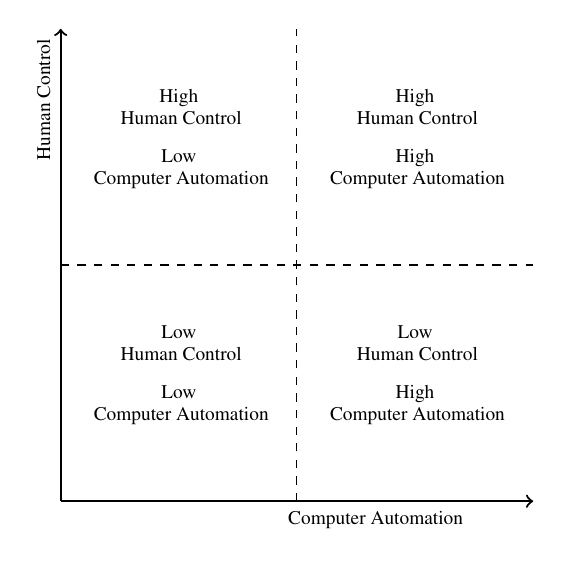
\begin{tikzpicture}[scale=0.6]
    \draw[->, thick] (0,0) -- (10,0) node[anchor=north, xshift=-2cm]
        {\scriptsize Computer Automation};
    \draw[->, thick] (0,0) -- (0,10) node[anchor=south east, rotate=90]
        {\scriptsize Human Control};
    \draw[dashed] (0,5) -- (10,5);
    \draw[dashed] (5,0) -- (5,10);
    \node[align=center, font=\scriptsize] at (2.5,2.5) {Low \\
        \vspace{0.2cm} Human Control \\ Low \\
        \vspace{0.2cm} Computer Automation};
    \node[align=center, font=\scriptsize] at (7.5,2.5) {Low \\
        \vspace{0.2cm} Human Control \\ High \\
        \vspace{0.2cm} Computer Automation};
    \node[align=center, font=\scriptsize] at (2.5,7.5) {High \\
        \vspace{0.2cm} Human Control \\ Low \\
        \vspace{0.2cm} Computer Automation};
    \node[align=center, font=\scriptsize] at (7.5,7.5) {High \\
        \vspace{0.2cm} Human Control \\ High \\
        \vspace{0.2cm} Computer Automation};
\end{tikzpicture}
}
\end{figure*}

This duality is articulated around three human control criteria ---ease of use, pipeline configurability and information comprehensibility--- and six automation criteria ---data type detection, data cleaning, feature engineering, model training, hyperparameter optimization and model validation---, forming an evaluative framework applicable to concrete tools. Among the risks that \gls{hcai} seeks to mitigate are algorithmic bias, frequently caused by imbalanced training data, and the lack of transparency inherent to systems that operate as black boxes \cite{chen2023human}.

\subsection{AutoML: Automation of the ML Pipeline}

\Gls{automl} tools emerged in response to the growing demand for \gls{ml} solutions and the shortage of qualified data scientists \cite{he2021automl}. Their purpose is to democratize access to \gls{ml} by automating complex tasks such as feature engineering, model selection, hyperparameter optimization and evaluation, making advanced analytics accessible to users without deep technical knowledge.

However, this predominantly automation-oriented approach frequently operates as a black box, making it difficult for users to understand decision-making processes, incorporate domain-specific knowledge or maintain meaningful control over the modeling process \cite{garouani2023unlocking}. This limitation is not minor: the lack of transparency can conceal underlying biases and prevent the human-AI collaboration necessary to obtain reliable and contextually appropriate results \cite{komala2024fair}.

The current market offers both commercial solutions ---such as Google \gls{automl}, Azure Automated \gls{ml} or Amazon SageMaker Autopilot--- and free alternatives ---including Ludwig, AutoGluon, H2O-3 or PyCaret---, designed to meet varying levels of technical expertise. However, the analysis of these tools under \gls{hcai} criteria reveals that none simultaneously maximizes human control and automation, each representing a different balance between accessibility, interpretability and technical sophistication \cite{palazuelos2024non}.

\subsection{Human-Guided Machine Learning}

\Gls{hgml} constitutes the practical realization of \gls{hcai} principles within the \gls{ml} domain \cite{gil2019towards}. Its fundamental premise is that the active participation of domain experts throughout the \gls{ml} pipeline is not only possible but beneficial, enriching the process with contextual knowledge that algorithms alone cannot incorporate. While \gls{automl} efficiently searches for solutions, expert input through intuitive interfaces enhances the process, resulting in more accurate, efficient and interpretable models \cite{lindauer2024position}.

Within the \gls{hgml} framework, this participation is structured around three main areas. In the data preparation phase, users can intervene in variable selection and transformation, the definition of subpopulations of interest and the management of outliers. During model development, the expert can guide the selection of algorithm families, impose constraints on parameters and influence pipeline design. Finally, in the results interpretation phase, users can request specific metrics, compare alternative configurations and analyze model sensitivity to parameter variations.

Despite its potential, existing \gls{hgml} proposals present notable limitations in practice. Although some theoretical frameworks cover specific parts of the pipeline, few offer complete software implementations accessible to users without \gls{ai} training \cite{lindauer2024position}, considerably reducing their applicability in real-world contexts.

\subsection{HCAI Criteria as an Evaluation Framework}

Despite the proliferation of \gls{automl} tools, their systematic evaluation under \gls{hcai} criteria remains infrequent. Most comparative studies focus on predictive performance metrics, relegating to the background aspects such as usability for non-expert users, the transparency of automated decisions or the actual degree of control the system grants to the user \cite{hartikainen2022human}.

Applying \gls{hcai} criteria as an evaluative framework allows going beyond performance and answering questions such as: in which pipeline phases does the user have real intervention capacity?, which decisions remain opaque or beyond their reach?, how are responsibilities distributed between the human and the system? This type of analysis is particularly valuable for guiding the design of future tools toward a more balanced and transparent human-machine collaboration, and represents a line of work explicitly called for by the research community \cite{lindauer2024position,wu2022survey}.

However, a critical limitation persists: the \gls{hcai} frameworks available in the literature ---including Shneiderman's two-dimensional model \cite{shneiderman2022human}--- are formulated at a level of abstraction that does not translate directly into operational evaluation instruments for \gls{hgml} tools. They define desirable properties but do not specify \textit{how} to assess them in the context of a concrete \gls{ml} pipeline, \textit{which} phases to examine, or \textit{what} criteria determine whether a given decision genuinely belongs to the user or to the automated system. Existing \gls{hgml} proposals \cite{gil2019towards,lindauer2024position} similarly lack evaluation instruments: they establish participation frameworks but provide no methodology for measuring the degree to which a tool actually realizes human-centered principles. This gap between conceptual frameworks and operational evaluation methodology is precisely what the present work seeks to address.


\section{\uppercase{A Methodology for Evaluating HGML Tools under HCAI Criteria}}
\label{sec:methodology}

\subsection{Motivation and Scope}

The absence of a principled evaluation methodology for \gls{hgml} tools constitutes a structural gap in the literature. While the \gls{hcai} framework provides a valuable conceptual foundation, its direct application to \gls{hgml} tools is non-trivial: the two-dimensional model of human control and computer automation must be operationalized in terms of concrete pipeline phases, decision types and responsibility assignment criteria before it can yield reproducible and comparable evaluations. The methodology proposed here addresses this need, providing a reusable instrument applicable to any \gls{hgml} tool regardless of its underlying technical implementation.

\subsection{Evaluation Dimensions}

The methodology is structured around the two independent dimensions of the \gls{hcai} framework \cite{shneiderman2022human}, each decomposed into measurable criteria specific to the \gls{hgml} domain:

\textbf{Human control dimension} is assessed through three criteria: (i) \textit{ease of use}, examining whether the tool can be operated by users without \gls{ai} expertise through its interface design and interaction patterns; (ii) \textit{pipeline configurability}, measuring the extent to which users can customize key decisions across pipeline phases without requiring code-level intervention; and (iii) \textit{information interpretability}, evaluating whether the system communicates its decisions, configurations and results in language and formats accessible to non-technical users.

\textbf{Computer automation dimension} is assessed through six criteria corresponding to the core technical tasks of the \gls{ml} pipeline: (i) \textit{data type detection}, (ii) \textit{data cleaning}, (iii) \textit{feature engineering}, (iv) \textit{model training}, (v) \textit{hyperparameter optimization} and (vi) \textit{model validation}. For each criterion, the evaluation determines whether the task is performed autonomously by the system, requires user intervention, or involves a shared responsibility.

\subsection{Pipeline Phase Framework}

The evaluation covers nine phases organized into three areas, following the \gls{hgml} framework of Gil et al. \cite{gil2019towards} as extended by Lindauer et al. \cite{lindauer2024position}:

\begin{itemize}
    \item \textbf{Data use:} variable selection, variable requirements and instance selection.
    \item \textbf{Model development:} model selection, parameter settings and solution design.
    \item \textbf{Model interpretation:} model assessment, model comparison and parameter comparison.
\end{itemize}

This phase structure ensures that the evaluation covers the complete \gls{ml} lifecycle, from raw data ingestion to actionable model insights, and provides a common reference frame for comparing different \gls{hgml} tools.

\subsection{Responsibility Assignment Criteria}

The central analytical operation of the methodology is the assignment of each decision within a pipeline phase to one of three responsibility categories:

\begin{itemize}
    \item \textbf{User responsibility:} decisions that require domain knowledge, contextual judgment or value-laden choices that cannot be derived from data alone (e.g., which variables are semantically relevant, what level of prediction error is acceptable for the application).
    \item \textbf{System responsibility:} decisions that require technical \gls{ml} expertise, computational search or statistical procedures that would be inaccessible or impractical for non-expert users (e.g., hyperparameter optimization, neural architecture selection, cross-validation).
    \item \textbf{Shared responsibility:} decisions where the user provides high-level guidance or constraints and the system executes within those bounds (e.g., the user selects preferred evaluation metrics; the system computes and reports them).
\end{itemize}

A tool achieves the \gls{hcai} target quadrant ---high human control and high computer automation--- when domain-knowledge decisions are consistently assigned to the user, technical decisions are consistently automated, and the interface makes the boundary between both categories explicit and comprehensible.

\subsection{The HCAI-HGML Compliance Matrix}

The methodology is formalized through the \gls{hcai}-\gls{hgml} Compliance Matrix, which crosses the nine pipeline phases (rows) against the nine \gls{hcai} evaluation criteria (columns): three human control criteria and six automation criteria. For each cell, the matrix records whether the tool \textbf{fully meets} the criterion in that phase (\checkmark), \textbf{partially meets} it ($\sim$), or \textbf{does not meet} it ($\times$).

This structure serves two purposes. First, it makes the evaluation systematic and reproducible: any evaluator applying the same criteria to the same tool should arrive at equivalent results. Second, it makes the evaluation \textit{comparable across tools}: by applying the matrix to different \gls{hgml} proposals, it becomes possible to identify which phases and which criteria are most frequently underserved in the current landscape, guiding future design efforts toward the most critical gaps.

Table~\ref{tab:compliance_matrix} presents the \gls{hcai}-\gls{hgml} Compliance Matrix as applied to \gls{insuml}, whose results are discussed in detail in Section~\ref{sec:hcai_evaluation}.

\begin{table*}[h]
\caption{\gls{hcai}-\gls{hgml} Compliance Matrix applied to \gls{insuml}. Human control criteria: EU = Ease of Use, PC = Pipeline Configurability, II = Information Interpretability. Automation criteria: DT = Data Type Detection, DC = Data Cleaning, FE = Feature Engineering, MT = Model Training, HO = Hyperparameter Optimization, MV = Model Validation. \checkmark = fully met; $\sim$ = partially met; $\times$ = not met.}
\label{tab:compliance_matrix}
\centering
\resizebox{\linewidth}{!}{%
\begin{tabular}{l ccc cccccc}
\toprule
 & \multicolumn{3}{c}{\textbf{Human Control}} & \multicolumn{6}{c}{\textbf{Automation}} \\
\cmidrule(lr){2-4} \cmidrule(lr){5-10}
\textbf{Pipeline phase} & \textbf{EU} & \textbf{PC} & \textbf{II} & \textbf{DT} & \textbf{DC} & \textbf{FE} & \textbf{MT} & \textbf{HO} & \textbf{MV} \\
\midrule
Variable selection      & \checkmark & \checkmark & \checkmark & \checkmark & $\sim$ & $\sim$ & --- & --- & --- \\
Variable requirements   & \checkmark & \checkmark & \checkmark & \checkmark & \checkmark & --- & --- & --- & --- \\
Instance selection      & \checkmark & $\sim$     & \checkmark & --- & \checkmark & --- & --- & --- & \checkmark \\
Model selection         & \checkmark & $\sim$     & $\sim$     & --- & --- & --- & \checkmark & \checkmark & --- \\
Parameter settings      & \checkmark & $\sim$     & \checkmark & --- & --- & --- & \checkmark & \checkmark & --- \\
Solution design         & \checkmark & $\sim$     & \checkmark & --- & \checkmark & \checkmark & \checkmark & --- & --- \\
Model assessment        & \checkmark & \checkmark & \checkmark & --- & --- & --- & --- & --- & \checkmark \\
Model comparison        & \checkmark & \checkmark & \checkmark & --- & --- & --- & --- & --- & \checkmark \\
Parameter comparison    & \checkmark & $\sim$     & \checkmark & --- & --- & --- & --- & \checkmark & \checkmark \\
\bottomrule
\end{tabular}%
}
\end{table*}

\subsection{Evaluation Procedure}

The application of the methodology to a given \gls{hgml} tool proceeds in four steps:

\begin{enumerate}
    \item \textbf{Interface walkthrough:} a systematic traversal of the tool's complete workflow, documenting every decision point encountered by the user and every automated action performed by the system.
    \item \textbf{Phase-by-phase responsibility mapping:} for each of the nine pipeline phases, decisions are classified according to the responsibility assignment criteria defined above, producing a structured responsibility distribution table.
    \item \textbf{Compliance Matrix completion:} the three human control criteria and six automation criteria are evaluated based on the evidence collected during the interface walkthrough, populating the \gls{hcai}-\gls{hgml} Compliance Matrix and yielding a structured profile of the tool's \gls{hcai} compliance.
    \item \textbf{Quadrant positioning:} the aggregated evidence from the matrix is used to position the tool within the \gls{hcai} two-dimensional framework, characterizing the overall balance achieved between human control and computer automation.
\end{enumerate}

This procedure is designed to be applicable by \gls{hci} researchers and practitioners without requiring access to the tool's source code, making it suitable for both internal evaluation during design and external comparative assessment across tools.



\section{\uppercase{InsuML: Tool Description}}
\label{sec:tool_description}

\subsection{Overview, Design Principles and Interface}

\Gls{insuml} is a software application designed to facilitate the construction of predictive models by users without \gls{ai} expertise. Its design rests on a central premise: that domain knowledge and expert intuition are valuable assets that must be explicitly integrated into the \gls{ml} process, rather than being displaced by automation. To this end, the tool adopts the \gls{hgml} paradigm as its structuring principle, combining the power of an \gls{automl} engine with a guided \gls{gui} that makes every pipeline decision visible and controllable \cite{shneiderman2022human}.

The interface is organized through a tab-based navigation system that guides users sequentially through the complete \gls{ml} pipeline without requiring programming skills. The workflow begins with a welcome screen that contextualizes the process, followed by dedicated tabs for dataset loading, variable configuration, training parameter selection and results visualization. Figure~\ref{fig:interface} shows the feature configuration tab, illustrating the dataset preview, variable assignment controls and missing value handling options.

% Figure~\ref{fig:interface}

During the configuration phase, users can remove irrelevant variables, assign input or output roles to each column, select evaluation metrics and define strategies for handling missing values. Before training begins, the system presents a summary of all selected options alongside applied default values, offering the user a complete and transparent view of the configuration to be executed. Once training is complete, results are presented through interactive graphics and confusion matrices that facilitate interpretation without requiring advanced statistical expertise. This design transforms habitually opaque technical decisions into explicit and comprehensible choices for the user, addressing one of the most frequent criticisms directed at conventional \gls{automl} systems \cite{garouani2023unlocking}.

\subsection{Architecture}

\Gls{insuml} is built on three modular layers: an Interface Layer implemented in Python using Tkinter, which manages user interaction and input validation; a Core Logic Layer that translates user selections into technical configurations and automatically generates the necessary configuration files; and an \gls{automl} Layer based on the Ludwig engine, which handles training, hyperparameter optimization and model evaluation autonomously. This separation ensures that all automated decisions can be traced and understood, contributing to bias mitigation and responsible \gls{ai} deployment \cite{chen2023human}. The modular design also allows the underlying \gls{automl} engine to be replaced without altering the user experience, ensuring flexibility and longevity.



\section{\uppercase{HCAI Evaluation of InsuML}}
\label{sec:hcai_evaluation}

This section applies the evaluation methodology proposed in Section~\ref{sec:methodology} to \gls{insuml}. The objective is to demonstrate the practical utility of the methodology while simultaneously characterizing the extent to which \gls{insuml} materializes the principles of the \gls{hcai} framework, examining how responsibilities are distributed between the user and the automated system throughout the different phases of the \gls{ml} pipeline.

\subsection{Application of the Methodology to InsuML}

The evaluation follows the four-step procedure defined in Section~\ref{sec:methodology}. The interface walkthrough was conducted through a complete traversal of \gls{insuml}'s tab-based workflow, from dataset loading to results visualization, documenting all decision points and automated actions. The resulting responsibility mapping covers the nine pipeline phases organized into the three areas of data use, model development and model interpretation, following the phase framework of Gil et al.~\cite{gil2019towards} and Lindauer et al.~\cite{lindauer2024position}.

\subsection{Human Control throughout the Pipeline}

\textbf{Data use.} In the variable selection phase, the user exercises direct and explicit control: they can review the complete dataset, identify irrelevant variables for their specific problem and remove them before training. This domain knowledge-based prioritization capability is precisely the type of intervention that conventional \gls{automl} systems do not contemplate. Regarding variable requirements, the user can explicitly designate which columns will act as input variables and which will be the target variable, as well as specify the problem type ---classification or regression---. Instance selection, in turn, allows the user to define treatment strategies for missing values, choosing between the removal of incomplete rows or imputation by column mean, a decision with direct implications for the quality and representativeness of the resulting model.

\textbf{Model development.} Model type selection is delegated to the Ludwig engine, which automatically chooses the most appropriate architecture based on dataset characteristics and problem type. However, the user can indirectly influence this through the configuration of training parameters, such as maximum training time or preferred evaluation metrics. Solution design remains partially in the user's hands through the preprocessing decisions made in earlier phases, whose impact on the complete pipeline is visible thanks to the configuration summary the system presents before training begins.

\textbf{Model interpretation.} Once training is complete, \gls{insuml} presents results through interactive visualizations including learning curves, confusion matrices and performance metrics adapted to the task type. This set of resources facilitates the user evaluating the model from their domain perspective, identifying error patterns and making informed decisions about whether the model is suitable for their application. The possibility of reconfiguring the pipeline and retraining the model also enables an implicit comparison between alternative configurations, fostering the iterative exploration characteristic of the \gls{hgml} approach.

\subsection{Pipeline Automation}

The Ludwig engine autonomously manages a broad set of technical tasks that would otherwise require advanced expertise. Automatic data type detection allows the system to infer whether each variable is numerical, categorical or of another type, applying appropriate encoders and transformations without user intervention. Data cleaning, beyond the user-configurable options, includes automatic normalization mechanisms and categorical variable encoding. Model training is executed entirely in an automated fashion, including neural architecture selection, hyperparameter optimization within predefined ranges and validation using standard techniques. All of this occurs transparently for the user, who receives continuous feedback on training progress without needing to intervene in the technical details.

\subsection{Balance between Human Control and Automation}

Table~\ref{tab:balance} synthesizes the distribution of responsibilities between the user and the system across the nine pipeline phases, illustrating the balance achieved by \gls{insuml} between human control and automation.

\begin{table*}[h]
\caption{Distribution of responsibilities between user and system in each
phase of the \gls{ml} pipeline in \gls{insuml}.}
\label{tab:balance}
\centering
\resizebox{\linewidth}{!}{%
\begin{tabular}{l p{6cm} p{6cm}}
\toprule
\textbf{Pipeline phase} & \textbf{Human control} & \textbf{Automation} \\
\midrule
Variable selection & The user prioritizes variables, proposes new combinations,
adjusts context and identifies missing data & The system infers relevant
features and performs automatic imputation during preprocessing \\
Variable requirements & The expert specifies inclusion or exclusion of
variables based on domain knowledge of their predictive strength & The system
enforces include/exclude rules defined in the configuration and validates
dataset consistency \\
Instance selection & The user defines subpopulations, selects or removes
outliers and sets the partitioning strategy & The system performs automatic
dataset splitting, balancing and cross-validation by default \\
Model selection & The user indicates preferred model types & The system builds
and evaluates candidate architectures \\
Parameter settings & The expert specifies parameter values based on domain
knowledge & The system searches and optimizes hyperparameters within declared
ranges \\
Solution design & The user modifies preprocessing, feature generation,
imputation and pipeline design & The system constructs complete pipelines
(encoders, combiners, preprocessing) \\
Model assessment & The user requests specific metrics & The system computes
and reports metrics, training curves and diagnostics automatically \\
Model comparison & The user selects models, datasets or configurations to
compare & The system manages multiple experiments and provides comparative
results and visualizations \\
Parameter comparison & The user identifies parameters for targeted variation &
The system runs ablation or sensitivity tests on parameter variations and
reports performance impact \\
\bottomrule
\end{tabular}%
}
\end{table*}

The analysis reveals that \gls{insuml} achieves a genuine balance between both dimensions. Decisions requiring domain knowledge ---which variables are relevant, what type of problem is being addressed, what level of error is acceptable--- fall explicitly on the user. Tasks demanding technical \gls{ml} expertise ---hyperparameter optimization, architecture selection, cross-validation--- are managed autonomously by the system. This distribution is not coincidental but the result of deliberate design decisions oriented toward placing the tool in the high automation and high human control quadrant of the \gls{hcai} framework \cite{shneiderman2022human}.

\subsection{Evaluation of Transversal Criteria}

Beyond the phase-by-phase analysis, the evaluation of the \gls{hcai} framework's transversal criteria offers a complementary view of the degree of compliance with human-centered design principles.

Regarding \textbf{ease of use}, the tab-based guided navigation, the absence of programming requirements and the progressive presentation of options significantly reduce the entry barrier for users without technical training. Automatic input validation and the comprehensible error messaging system further contribute to a robust and accessible user experience.

With respect to \textbf{pipeline configurability}, \gls{insuml} offers a medium-high level of flexibility. Users can customize key aspects of the process ---variables, metrics, imputation strategies, training time--- without needing to modify code. However, the dependency on the Ludwig engine imposes limitations on the configuration of model architectures at a low level, an aspect that represents a future improvement opportunity.

Regarding \textbf{information interpretability}, the system presents results through interactive visualizations and accessible language, avoiding the direct exposure of technical parameters to the user. The pre-training configuration summary is a particularly valuable element, as it allows the user to verify and understand exactly what process will be executed before initiating it, transforming automated decisions into transparent and verifiable options \cite{garouani2023unlocking}.


\section{\uppercase{Discussion}}
\label{sec:discussion}

\subsection{InsuML in the AutoML and HGML Landscape}

The \gls{hcai} evaluation presented in the previous section allows \gls{insuml} to be situated within the current \gls{automl} landscape from a perspective that goes beyond predictive performance. Tools such as AutoGluon or H2O-3 achieve more competitive results on most benchmarks, but their predominant orientation toward technically proficient users, the absence of guided workflows and the limited interpretability of their interfaces place them in a design space different from that advocated by \gls{hcai} \cite{lindauer2024position}. \Gls{insuml} does not compete in the same space as these tools: it competes in the human-centered design space, where accessibility, transparency and meaningful control are the primary success criteria.

The comparison with existing \gls{hgml} proposals further reinforces this distinction. Works such as those of Gil et al. \cite{gil2019towards} and Lee et al. \cite{lee2020human} establish comprehensive theoretical frameworks covering the full \gls{ml} pipeline from a human-centered perspective, but lack software implementation and have not been evaluated under \gls{hcai} criteria. The HAMLET framework of Francia et al. \cite{francia2023hamlet}, while providing partial software support, is specifically oriented toward \gls{ai} experts, limiting its applicability to the non-technical user profile that \gls{hgml} aims to reach. Lindauer et al. \cite{lindauer2024position} explicitly call for more human-centered \gls{automl} tools, acknowledging that current proposals insufficiently address usability, interpretability and customization criteria. \Gls{insuml} is the only proposal that combines full pipeline coverage, operational software implementation, accessibility for non-AI users and explicit evaluation under \gls{hcai} criteria.

\subsection{Prospective Transparency as a Design Principle}

A concept that emerges from the evaluation of \gls{insuml} and deserves explicit articulation is what we term \textit{prospective transparency}: the capacity of a system to make its forthcoming automated behavior visible and verifiable to the user \textit{before} that behavior is executed, rather than explaining it \textit{after the fact}. This concept is distinct from the post-hoc explainability that dominates the \gls{xai} literature \cite{salih2025perspective}, and represents a complementary and arguably more preventive approach to the transparency problem in \gls{ml} systems.

In \gls{insuml}, prospective transparency is materialized through the pre-training configuration summary: a checkpoint that presents the complete set of user-selected options and system-applied defaults before training begins. This mechanism transforms the transition from user configuration to automated execution ---habitually an opaque boundary in conventional \gls{automl} systems--- into an explicit verification step. The user is not merely informed of what the system did; they are invited to confirm what the system \textit{will do}, preserving their agency at the most consequential decision point in the pipeline. This design principle directly addresses the transparency deficit identified as one of the main shortcomings of current \gls{automl} systems \cite{garouani2023unlocking}, and constitutes a transferable pattern for the design of future \gls{hgml} tools.

\subsection{Design Implications for Accessible ML Interfaces}

The \gls{hcai} evaluation of \gls{insuml} yields transferable insights for the design of future \gls{ml} tools targeting non-expert users. First, sequential tab-based navigation proves to be an effective interaction pattern for guiding users through complex processes without overwhelming them with simultaneous technical options. The structured progression reduces cognitive load and allows users to focus on domain decisions while delegating technical ones to the system.

Second, the pre-training configuration summary ---discussed above as a prospective transparency mechanism--- emerges as a particularly valuable design element from the \gls{hcai} perspective, directly addressing the transparency deficit identified as one of the main shortcomings of current \gls{automl} systems \cite{garouani2023unlocking}.

Third, the architectural separation between the interface and core logic layers carries ethical implications beyond its technical advantages. By making the translation between user intentions and technical parameters explicit, the system reduces the risk of inadvertent perpetuation of data biases, a problem frequently highlighted in the responsible \gls{ai} literature \cite{chen2023human,komala2024fair}.

\subsection{Limitations and Future Work}

The evaluation presented in this work is not without limitations. Although \gls{insuml} was co-designed with non-expert users, the current work lacks formal usability studies measuring empirical metrics such as task completion time, error rates or user satisfaction with actual domain specialists performing realistic modeling tasks. This empirical validation constitutes the most immediate priority for future work, and should be conducted following established \gls{hci} research methods \cite{lazar2017research}.

Additionally, \gls{insuml}'s current explainability capabilities are limited. Incorporating \gls{xai} techniques such as \gls{shap} or \gls{lime} \cite{salih2025perspective} would considerably enrich the model interpretation phase, enabling users to understand not only global model performance but also which variables contribute to each prediction and why. Finally, experiments have been restricted to moderately sized datasets in structured tabular format; extending the tool toward larger-scale datasets and heterogeneous data sources ---text, images, time series--- would significantly broaden its real-world applicability while maintaining the human-centered design principles that articulate its development.



\section{\uppercase{Conclusions}}
\label{sec:conclusions}

This paper has presented two interrelated contributions. First, a structured methodology for evaluating \gls{hgml} tools under \gls{hcai} criteria, which operationalizes the two-dimensional \gls{hcai} framework into concrete pipeline phases, responsibility assignment criteria and a reproducible four-step evaluation procedure formalized as an \gls{hcai}-\gls{hgml} Compliance Matrix. Second, an application of this methodology to \gls{insuml}, an \gls{hgml} tool designed for users without \gls{ai} expertise, with the objective of analyzing the extent to which it simultaneously materializes high levels of automation and meaningful human control.

The results of the analysis demonstrate that \gls{insuml} achieves a genuine balance between both dimensions of the \gls{hcai} framework. Decisions requiring domain knowledge fall explicitly on the user, while tasks demanding advanced technical expertise are managed autonomously by the system. This distribution is not coincidental but the result of deliberate design decisions, manifested in concrete interface elements such as tab-based guided navigation, the pre-training configuration summary ---which instantiates the principle of prospective transparency--- and the presentation of results through accessible visualizations.

The comparison with existing \gls{hgml} proposals reveals that \gls{insuml} is the only one that combines full pipeline coverage, operational software implementation, accessibility for users without \gls{ai} training and explicit evaluation under \gls{hcai} criteria. This combination represents a concrete contribution to the democratization of \gls{ml}, not only in terms of technical capabilities but also in terms of responsibility: by making every process decision visible and controllable, the tool enables domain experts to apply their contextual knowledge to prevent problematic algorithmic behaviors.

From the \gls{hci} perspective, this work illustrates that interface design for \gls{ml} systems is not a secondary concern but a determining factor for human-AI collaboration to be effective and responsible. Interface design decisions ---how options are presented, in what order, with what level of technical detail--- have direct implications for the degree of real control the user exercises over the system and, by extension, for the quality and reliability of the resulting models.

As future work, the most immediate priority is conducting formal usability studies with real users from different domains \cite{lazar2017research}, to empirically validate whether the current design achieves its accessibility and control objectives. The incorporation of advanced explainability techniques and the extension toward heterogeneous data sources represent complementary development lines that would broaden the scope and applicability of the tool, maintaining human-centered design principles as the articulating axis throughout.

In summary, this work contributes on two fronts: it proposes a reusable evaluation methodology that fills a gap identified in the \gls{hcai} and \gls{hgml} literature, and it demonstrates through its application to \gls{insuml} that high automation and high human control are not opposing objectives but complementary ones when interaction design is approached with rigor and with the non-expert user as the protagonist.


\section*{\uppercase{Acknowledgements}}

This work has been supported by grant PID2023-146243OB-I00 funded by MICIU/AEI/10.13039/501100011033 and by ``ERDF/EU''.


\bibliographystyle{apalike}
{\small
\bibliography{bibliography}}

\end{document}

